\documentclass[a4paper,oneside,DIV=12,12pt,headings=normal]{scrartcl}

%%% Length calculations
\usepackage{calc}
%%%

%%% Support for color
\usepackage{xcolor}
\definecolor{lightblue}{HTML}{03A9F4}
\definecolor{red}{HTML}{F44336}
%%%

%%% Graphics inclusion
\usepackage{graphicx}
%%%

%%% Font selection
\usepackage{fontspec}

\setromanfont{STIX Two Text}[
]

\setsansfont{Source Sans Pro}[
]

\setmonofont{Source Code Pro}[
]

\usepackage{unicode-math}
\setmathfont{STIX Two Math}

%%%

%%% Font settings for different KOMA Script elements
\setkomafont{pagenumber}{\rmfamily}
\setkomafont{disposition}{\rmfamily\bfseries}
%%%

%%% Typographic enhancements
\usepackage{microtype}
%%%

%%% Language-specific settings
\usepackage{polyglossia}
\setmainlanguage{ukrainian}
%%%

%%% List settings
\usepackage{enumitem}
\setlist[enumerate]{
	leftmargin = *,
}
%%%

%%% Captions
\usepackage{caption}
\usepackage{subcaption}

\captionsetup{
	% format = plain,
	% labelfont = bf,
	% justification = raggedright,
}

\DeclareCaptionLabelFormat{closing}{#2)}
\captionsetup[subtable]{labelformat = closing}
\captionsetup[subfigure]{labelformat = closing, position = auto}
%%%

%%% Tables
\usepackage{booktabs}
% \usepackage{longtable}

\usepackage{multirow}

\usepackage{array}
\newcolumntype{v}[1]{>{\raggedright\arraybackslash\hspace{0pt}}p{#1}}
\newcolumntype{b}[1]{>{\centering\arraybackslash\hspace{0pt}}p{#1}}
\newcolumntype{n}[1]{>{\raggedleft\arraybackslash\hspace{0pt}}p{#1}}
%%%

%%% Floats on a single row
\usepackage{floatrow}
\newfloatcommand{capbtabbox}{table}[][\FBwidth]
%%%

%%% Links and hyperreferences
\usepackage{hyperref}
\hypersetup{
	colorlinks      = false,
	linkbordercolor = red,
	urlbordercolor  = lightblue,
	pdfborderstyle  = {/S/U/W 1.5},
}
%%%

%%% All caps
\newcommand{\allcaps}[1]{{\addfontfeatures{LetterSpace = 3}#1}}
%%%


\begin{document}
	\begin{titlepage}
	\centering
		Міністерство освіти і науки України\\
		Національний авіаційний університет\\
		Навчально-науковий інститут комп'ютерних інформаційних технологій\\
		Кафедра комп'ютеризованих систем управління

		\vspace*{\fill}

		Лабораторна робота №1\\
		з дисципліни «Комп'ютерна схемотехніка»\\
		на тему «Дослідження дешифраторів і шифраторів»

		\vspace*{\fill}
		
		\begin{flushright}
			Виконав:\\
			студент ННІКІТ СП-225\\
			Клокун В.\,Д.\\
			Перевірив:\\
			Іскренко Ю.\,Ю.
		\end{flushright}

		Київ 2018
    \end{titlepage}
	
	\section{Мета роботи}
		% \begin{enumerate}
			% \item Вивчення принципів побудови, логіки роботи й синтезу дешифраторів і шифраторів.
			% \item Освоєння методики дослідження схем дешифраторів і шифраторів.
			% \item Визначення основних характеристик і параметрів дешифраторів і шифраторів на інтегральних мікросхемах.
			% \item Ознайомлення з мікросхемами дешифраторів та шифраторів вітчизняних серій \allcaps{ТТЛШ}, \allcaps{ЕЗЛ}, \allcaps{КМОН}.
		% \end{enumerate}
		
		Вивчення принципів побудови, логіки роботи й синтезу дешифраторів і шифраторів. Освоєння методики дослідження схем дешифраторів і шифраторів. Визначення основних характеристик і параметрів дешифраторів і шифраторів на інтегральних мікросхемах.
			
	\section{Хід роботи}
		\subsection{Дослідження лінійного дешифратора на~2~входи і~4~інверсні виходи на елементах І—НЕ}
			Складаємо схему лінійного дешифратора на 2~входи і 4~інверсні виходи на елементах І—НЕ (рис.~\ref{fig:00-schematic-linear-2in-4out-inv}). За результатами експерименту заповнюємо таблицю істинності (табл.~\ref{tab:00-linear-2in-4out-inv-truthtable}).
			
			\begin{figure}[!htbp]
				\begin{floatrow}
					\ffigbox[\Xhsize/2]{
						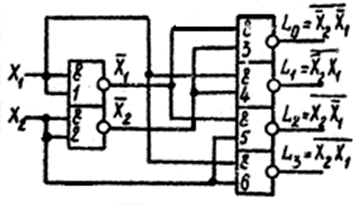
\includegraphics[height = 6\baselineskip]{./assets/00.png}
					}{
						\caption{Схема лінійного дешифр. на~2~входи і~4~інверсні виходи}
						\label{fig:00-schematic-linear-2in-4out-inv}
					}
					\capbtabbox[\Xhsize]{
						\begin{tabular}{*{6}{c}}
							\toprule
								$X_2$ & $X_1$ & $L_0$ & $L_1$ & $L_2$ & $L_3$ \\
							\midrule
								0 & 0 & 0 & 1 & 1 & 1 \\
								0 & 1 & 1 & 0 & 1 & 1 \\
								1 & 0 & 1 & 1 & 0 & 1 \\
								1 & 1 & 1 & 1 & 1 & 0 \\
							\bottomrule
						\end{tabular}
					}{%
						\caption{Таблиця істинності лінійного дешифр. на~2~входи і~4~інв. виходи}
						\label{tab:00-linear-2in-4out-inv-truthtable}
					}
				\end{floatrow}
			\end{figure}
		
		\subsection{Дослідження лінійного дешифратора на~2~входи і~4~прямі виходи на елементах І—НЕ}
			Складаємо схему лінійного дешифратора на 2~входи і 4~прямі виходи на елементах І—НЕ (рис.~\ref{fig:01-schematic-linear-2in-4out}). За результатами експерименту заповнюємо таблицю істинності (табл.~\ref{tab:01-truthtable-linear-2in-4out}).
			
			\begin{figure}[!htbp]
				\begin{floatrow}
					\ffigbox[\Xhsize/2]{
						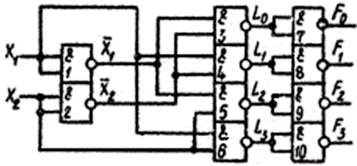
\includegraphics[height = 6\baselineskip]{./assets/01.png}
					}{
						\caption{Схема лінійного дешифр. на~2~входи і~4~прямі виходи}
						\label{fig:01-schematic-linear-2in-4out}
					}
					\capbtabbox[\Xhsize]{
						\begin{tabular}{*{6}{c}}
						\toprule
							$X_2$ & $X_1$ & $L_0$ & $L_1$ & $L_2$ & $L_3$ \\
						\midrule
							0 & 0 & 1 & 0 & 0 & 0 \\
							0 & 1 & 0 & 1 & 0 & 0 \\
							1 & 0 & 0 & 0 & 1 & 0 \\
							1 & 1 & 0 & 0 & 0 & 1 \\
						\bottomrule
					\end{tabular}
					}{
						\caption{Таблиця істинності лінійного дешифр. на~2~входи і~4~прямі виходи}
						\label{tab:01-truthtable-linear-2in-4out}
					}
				\end{floatrow}
			\end{figure}
			
		\subsection{Дослідження лінійного дешифратора на 2~входи і~4~прямі виходи зі стробними входами}
			Складаємо схему лінійного дешифратора на 2~входи і 4~прямі виходи зі стробними входами (рис.~\ref{fig:02-schematic-linear-2in-4out-strobe}). За результатами експерименту заповнюємо таблицю істинності (табл.~\ref{tab:02-truthtable-linear-2in-4out-strobe}).
			
			\begin{figure}[!htbp]
			\centering
				\begin{floatrow}
					\ffigbox[\Xhsize/2]{
						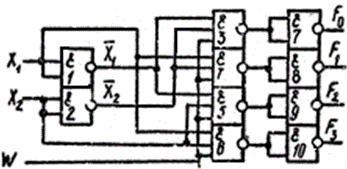
\includegraphics[height = 7\baselineskip]{./assets/02.png}
					}{
						\caption{Схема лінійного дешифр. на~2~входи і~4~прямі виходи зі~стробуванням}
						\label{fig:02-schematic-linear-2in-4out-strobe}
					}
					\capbtabbox[\Xhsize]{
						\begin{tabular}{*{7}{c}}
						\toprule
							$W$ & $X_2$ & $X_1$ & $F_0$ & $F_1$ & $F_2$ & $F_3$ \\
						\midrule
							0 & — & — & 1 & 0 & 0 & 0 \\
							1 & 0 & 0 & 1 & 0 & 0 & 0 \\
							1 & 0 & 1 & 0 & 1 & 0 & 0 \\
							1 & 1 & 0 & 0 & 0 & 1 & 0 \\
							1 & 1 & 1 & 0 & 0 & 0 & 1 \\
						\bottomrule
					\end{tabular}
					}{
						\caption{Таблиця істинності лінійного дешифр. на~2~входи і~4~прямі виходи зі~стробуванням}
						\label{tab:02-truthtable-linear-2in-4out-strobe}
					}
				\end{floatrow}
			\end{figure}
			
		\subsection{Дослідження пірамідального дешифратора на~3~входи і~8~прямих виходів}
			Складаємо схему пірамідального дешифратора на 3~входи і~8~прямих виходи (рис.~\ref{fig:03-schematic-pyramidal-3in-8out}). За результатами експерименту заповнюємо таблицю істинності (табл.~\ref{tab:03-truthtable-pyramidal-3in-8out}).
			
			\begin{figure}[!htbp]
			\centering
				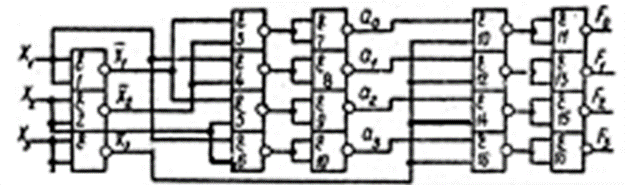
\includegraphics[height = 5\baselineskip]{./assets/03.png}
			\caption{Схема пірамідального дешифратора на 3~входи і 8~прямих виходи}
			\label{fig:03-schematic-pyramidal-3in-8out}
			\end{figure}
			
			\begin{table}[!htbp]
			\centering
				\begin{tabular}{*{14}{c}}
					\toprule
						$X_3$ & $X_2$ & $X_1$ & $F_0$ & $F_1$ & $F_2$ & $F_3$ & $V_3$ & $V_2$ & $V_1$ & $F_4$ & $F_5$ & $F_6$ & $F_7$ \\
					\midrule
						0 & 0 & 0 & 1 & 0 & 0 & 0 & 1 & 0 & 0 & 0 & 0 & 0 & 0 \\
						0 & 0 & 1 & 0 & 1 & 0 & 0 & 1 & 0 & 1 & 0 & 0 & 0 & 0 \\
						0 & 1 & 0 & 0 & 0 & 1 & 0 & 1 & 1 & 0 & 0 & 0 & 0 & 0 \\
						0 & 1 & 1 & 0 & 0 & 0 & 1 & 1 & 1 & 1 & 0 & 0 & 0 & 0 \\
					\bottomrule
				\end{tabular}
			\caption{Таблиця істинності пірамідального дешифратора на 3~входи і 8~прямих виходи}
			\label{tab:03-truthtable-pyramidal-3in-8out}
			\end{table}
			
		\subsection{Дослідження шифратора на~6~входів і~3~виходи на елементах І—НЕ}
			Складаємо схему пірамідального шифратора на 6~входів і~3~виходи на елементах І—НЕ (рис.~\ref{fig:04-schematic-linear-6in-3out}). За результатами експерименту заповнюємо таблицю істинності (табл.~\ref{tab:04-truthtable-linear-6in-3out}).
			
			\begin{figure}[!htbp]
			\centering
				\begin{floatrow}
					\ffigbox[\Xhsize/3]{
						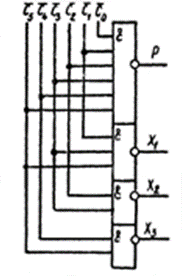
\includegraphics[height = 9\baselineskip]{./assets/04.png}
					}{
						\caption{Схема пі\-ра\-мі\-даль\-ного шифратора на 6~входів і 3~виходи}
						\label{fig:04-schematic-linear-6in-3out}
					}
					\capbtabbox[\Xhsize]{
						\begin{tabular}{*{10}{c}}
							\toprule
								$C_5$ & $C_4$ & $C_3$ & $C_2$ & $C_1$ & $C_0$ & $X_3$ & $X_2$ & $X_1$ & $P$ \\
							\midrule
								0 & 0 & 0 & 0 & 0 & 0 & 0 & 0 & 0 & 0 \\
								0 & 0 & 0 & 0 & 0 & 1 & 0 & 0 & 0 & 1 \\
								0 & 0 & 0 & 0 & 1 & 0 & 0 & 0 & 1 & 1 \\
								0 & 0 & 0 & 1 & 0 & 0 & 0 & 1 & 0 & 1 \\
								0 & 0 & 1 & 0 & 0 & 0 & 0 & 1 & 1 & 1 \\
								0 & 1 & 0 & 0 & 0 & 0 & 1 & 0 & 0 & 1 \\
								1 & 0 & 0 & 0 & 0 & 0 & 1 & 0 & 1 & 1 \\
							\bottomrule
						\end{tabular}
					}{
						\caption{Таблиця істинності пірамідального шифратора на 6~входів і 3~виходи}
						\label{tab:04-truthtable-linear-6in-3out}
					}
				\end{floatrow}
			\end{figure}
			
	\section{Висновок}
		Виконуючи дану лабораторну роботу, ми вивчили принципи побудови, логіки роботи й синтезу дешифраторів і шифраторів; освоїли методику дослідження схем дешифраторів і шифраторів; визначили основні характеристики і параметри дешифраторів і шифраторів на інтегральних мікросхемах.
		
\end{document}